\documentclass[7pt]{article}
\usepackage[utf8]{inputenc}
\usepackage[spanish]{babel}
\usepackage[rmargin=1.5cm, lmargin=1.5cm, tmargin= 2.5cm, bmargin=2.5cm]{geometry}
\usepackage[svgnames,x11names,dvipsnames]{xcolor} 
\usepackage{graphics}
\usepackage[rightcaption]{sidecap}
\usepackage{caption}
\usepackage{mathrsfs}
\usepackage{amssymb}
\usepackage{amsmath}
\usepackage{mathrsfs}
\usepackage{dsfont}
\usepackage{array}
\usepackage{amsfonts}
\usepackage{xcolor}
\usepackage{latexsym} %permite 
\usepackage{graphicx}
\usepackage{array}
\usepackage{multirow}
\usepackage{lipsum}
\usepackage{hyperref}
\usepackage{multicol} 
\usepackage{wrapfig}
\usepackage{hyperref} %hiperlinks
\newenvironment{Figura}
{\par\medskip\noindent\minipage{\linewidth}}
  {\endminipage\par\medskip}


\pagecolor{white} %color a la hoja
\color{black} %color de letra

%http://latexcolor.com/ 
%-----------CABECERA-----------------
\usepackage{fancyhdr}%paqueteria para modificar encabezados
\pagestyle{myheadings}
\pagestyle{fancy} %pone la paqueteria
%---------------------------------

\fancypagestyle{UltimaPagina}{
\fancyhead[C]{}
\fancyhead[L]{\footnotesize{MARTA BERHOLTS \emph{et al.}}} 
\fancyhead[R]{\footnotesize{PHYSICAL REVIEW RESEARCH \textbf{4}, 043041 (2022)}}
\fancyfoot[L]{}
\fancyfoot[C]{\footnotesize{043041-6}}
\fancyfoot[R]{}
} %Definí un estilo de página, con sus características propias, al empezar una página sólo pueden poner \thispagestyle{} para "pegar" el estilo de página acá definido, para que no haya errores raros en los estilos de página. Obviamente sólo funciona para un documento con pocas páginas.

 \fancypagestyle{Pagina3}{
\fancyhead[C]{}
\fancyhead[L]{\footnotesize{QUANTUM WATCH AND ITS INTRINSIC PROOF OF...}} 
\fancyhead[R]{\footnotesize{PHYSICAL REVIEW RESEARCH \textbf{4}, 043041 (2022)}}
\fancyfoot[L]{}
\fancyfoot[C]{\footnotesize{043041-3}}
\fancyfoot[R]{}
}

\hypersetup{
    colorlinks=true,
    urlcolor=blue,
    } %configura el estilo de las referencias e hiperlinks

\urlstyle{same}

\begin{document}
%--------------CABECERA--------
\newpage
\fancyhead[C]{PHYSICAL REVIEW RESEARCH \textbf{4}, 043041 (2022)}   
\fancyfoot[L]{ \footnotesize{2643-1564/2022/4(4)/043041(6)}}
\fancyfoot[C]{ \footnotesize{043041-1}}
\fancyfoot[R]{ \footnotesize{Published by the American Physical Society}}
%--------------------------------

\begin{center}
    \textbf{\Large{Quantum watch and its intrinsic proof of accuracy}}\\ 
\vspace{0.6cm}
\small{}
Marta Berholts,$^{\textcolor{Blue}{1,2,*}}$ Ronny Knut,$^{\textcolor{Blue}{1,\dag}}$ Robert Stefanuik,$^{\textcolor{Blue}{1}}$ Hampus Wikmark,$^{\textcolor{Blue}{1}}$ Susmita Saha,$^{\textcolor{Blue}{1,3}}$ and Johan Söderström$^{\textcolor{Blue}{1,\ddagger}}$.\\
Department of Physics and Astronomy, University of Uppsala, SE-75120 Uppsala, Sweden\\
Department of Physics, University of Tartu, EST-50411 Tartu, Estonia\\
Department of Physics, Ashoka University, IN-131029 Sonipat, India\\
\vspace{0.6cm}
(Received 25 January 2022; accepted 17 August 2022; published 18 October 2022)
\end{center}

\begin{center}
    \begin{minipage}{15cm}
    \small{}
        We have investigated the rich dynamics of complex wave packets composed of multiple high-lying Rydberg states in He. A quantitative agreement is found between theory and time-resolved photoelectron spectroscopy experiments. We show that the intricate time dependence of such wave packets can be used for investigating quantum defects and performing artifact-free timekeeping. The latter relies on the unique fingerprint that is created by the time-dependent photoionization of these complex wave packets. These fingerprints determine how much time has passed since the wave packet was formed and provide an assurance that the measured time is correct. Unlike any other clock, this quantum watch does not utilize a counter and is fully quantum mechanical in its nature. The quantum watch has the potential to become an invaluable tool in pump-probe spectroscopy due to its simplicity, assurance of accuracy, and ability to provide an absolute timestamp, i.e., there is no need to find time zero.\\ \\
    DOI:\textcolor{Blue}{\url{10.1103/PhysRevResearch.4.043041}}
    \end{minipage}
\end{center}
\hfill

\begin{multicols}{2}
\small{}
\begin{center}
    \section*{\normalsize{I. INTRODUCTION}}
\end{center}
A Rydberg wave packet (WP) consists of a coherent superposition of Rydberg states [1,2]. Unlike the single Rydberg state, the WP has a prominent time dependence in its radial wave function. The time evolution of the Rydberg WP is a result of wave-function interference between the different energy levels, and the number of Rydberg states in the WP will largely determine the complexity of its time dependence.
A WP of two Rydberg states will result in a harmonic oscillation in observed intensity. These basic Rydberg WPs are well studied [3–16]. However, if many Rydberg levels are excited, then a complex oscillatory pattern will emerge. We show that the complex time dependence can be utilized for investigating the theory-predicted quantum defect (QD), without explicitly measuring the energy of the Rydberg states. Furthermore, we show that the oscillations resulting from an ensemble of highly excited Rydberg states, that converge at the ionization threshold, give rise to a unique interference pattern that does not repeat during the lifetime of the WP (hundreds of ns) [17]. 
We refer to these oscillations as quasiunique beat signatures (QUBS), since they provide a fingerprint of how much time has evolved since the WP was created. Using the QUBS, we determine that our experimental setup has a drift of about 1 fs/ps when changing the path length of the pump beam using a delay stage. Unlike other clocks such as mechanical, quartz crystal, or atomic, which operate by counting\\
\rule{20mm}{0.1mm}\\
%---

    \begin{minipage}{7cm}
    \footnotesize{
        $^*$Corresponding author: marta.berholts@gmail.com\\
        $^{\dag}$ronny.knut@physics.uu.se\\
        $^{\ddagger}$johan.soderstrom@physics.uu.se}
    \end{minipage}\\ \\


\footnotesize{\textit{Published by the American Physical Society under the terms of the \textcolor{Blue}{Creative Commons Attribution 4.0 International} license. Further distribution of this work must maintain attribution to the author(s) and the published article’s title, journal citation, and DOI.}  }
 \\

%----
\small{}
the number of oscillations from a well-defined frequency, the QUBS-based timer does not utilize a counter. Instead, it provides a fingerprint representing a specific time and hence only requires interaction when initiating and reading out the time. Therefore, to separate it from the functionality of clocks, we will denote it as a “watch.” The main advantage of the quantum watch, compared to relying on a delay stage, is
that it effectively has no sources of systematic error, which is why we could determine the anomalous drift in our delay stage using QUBS. If there were any unknown external forces that affected the energy levels, giving a systematic error in the derived QUBS-time, then it would result in deviations between the measured and calculated QUBS. The fact that we have a quantitative agreement, indicates that there are no systematic errors and that the derived time is correct, or in other words, we have proof that the derived time is accurate. Such a quantum watch offers a unique opportunity to have an absolute timestamp without the necessity to measure time zero. First, this is crucial for pump-probe experiments to ensure that the delay stage is stable over time and, second, it could be used to find delay times when defining time zero is
not trivial. 

In this work, we created WPs composed of Rydberg states in the range from $n = 10 \longrightarrow \infty$ in He atoms, the electronic properties of which have been extensively investigated theoretically [18,19]. To monitor the temporal evolution of the WP we employed a pump-probe scheme. Helium was initially excited by an XUV pump pulse with appropriate energy and bandwidth and then photoionized by a time-delayed nearinfrared (NIR) probe pulse. The schematic of the investigated mechanism is shown in Fig. 1. As a result of using an XUV pulse centered around the He ionization potential, we observe three different ionization processes: ionization of the ground state electron by a single XUV pulse, direct twophoton ionization, and sequential photo-ionization [the latter is shown in Fig. 1(a)]. Direct two-photon ionization leads to



%--------------CABECERA--------
\newpage
\fancyhead[C]{ } 
\fancyhead[L]{\footnotesize{MARTA BERHOLTS \emph{et al.}}} 
\fancyhead[R]{\footnotesize{PHYSICAL REVIEW RESEARCH \textbf{4}, 043041 (2022)}}
\fancyfoot[L]{}
\fancyfoot[C]{ \footnotesize{043041-2}}
\fancyfoot[R]{ }
%--------------------------------
    \begin{Figura}
        \centering
        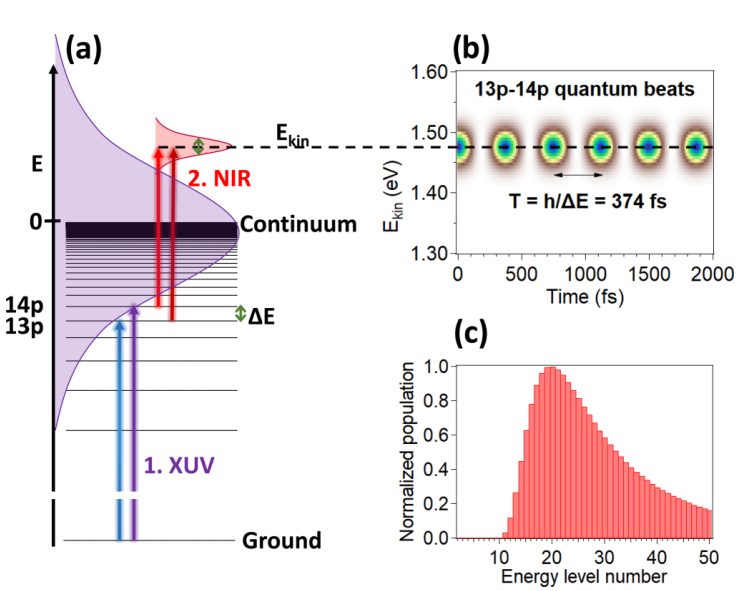
\includegraphics[scale=0.57]{Imagenes/2022-11-18.png}
    \end{Figura}
FIG. 1. (a) An ultrashort XUV pulse, shown in purple, with center energy close to the ionization threshold, is used for creating a coherent superposition of Rydberg states. Subsequently, an ultrashort NIR laser pulse, shown in red, ionizes the excited atom, resulting in photoelectrons with a kinetic energy of Ekin. (b) Simulation of quantum beats originating exclusively from the interference between levels He 1s13p 1P and He 1s14p 1P with energy separation of $E = 11 meV$. (c) After the XUV excitation, the WP consists of all energy levels between $n = 10$ and $\infty$.\\

so-called sidebands [20] that occur only during pump-probe overlap. Sequential photo-ionization is mediated by a resonant excitation below the continuum, and therefore the ionized photoelectron can be observed at times when the two pulses do not overlap in time but is limited to the lifetime of the Rydberg states. For He 1s10p 1P, the lifetime is in the order of 60 ns [17,21,22], and this becomes longer for higher Rydberg states. The temporal evolution of the phase of each Rydberg level in the coherently populated ensemble of excited states is proportional to the energy. The difference in phase evolution between various states can result in constructive and destructive interference of the signal intensity. This is illustrated in Fig. 1(b), where the photoelectrons from two Rydberg levels (13p and 14p) interfere, creating quantum beats with a frequency proportional to the levels’ binding energy difference.


In Fig. 1(c), we show the population of Rydberg states after the XUV excitation. Since the ground state is 1S state, the dipole approximation gives that the excited state is of 1 P character. In principle, all states above $n = 10$ are populated, but the absorption cross section decreases with increasing n, by n-3 $[23]$. Furthermore, the photoionization cross section of excited states also decreases with n-3 $[24]$, hence any levels above 50 have an insignificant contribution to the measured signal.

%----------
\small{}
    \begin{center}
        \section*{\normalsize{II. EXPERIMENT}}
    \end{center}
The experiment was performed at the HELIOS laboratory $[25,26]$. The setup consists of a commercial Ti:sapphire driving laser that produces 800 nm (1.55 eV) pulses with a
pulse duration of $\sim$45 fs. The laser output is split into two branches: Twenty percent of the fundamental laser beam is directly used as a NIR probe, while the remaining $80\%$ is used for the high harmonic generation (HHG) in an Ar-filled
gas cell to create the XUV pump. Due to symmetry reasons, the HHG process generally produces odd harmonics, but the ionization threshold of He (24.59 eV [19]) resides between the odd harmonics of 15 and 17. We hence generated even harmonics by using a BBO crystal for frequency doubling, which breaks the symmetry by mixing the electric field of 800 nm and 400 nm light [27–29]. At optimal phase matching (maximum fluence), the 16th harmonic has an energy of 24.8 eV. However, by adjusting the gas pressure and laser
intensity it is possible to shift the harmonic energy to 24.6 eV, corresponding to the He ionization threshold. A monochromator was used for selecting a fraction of 16th harmonic, the transmitted light had a bandwidth of about 0.1 eV.

After that, the XUV beam was directed to the interaction region where it spatially overlapped with the NIR probe beam. The intensity of the NIR beam at the interaction region was $\sim 9 x 1011$ W/cm2. The arrival time of the NIR pulse, relative to the XUV pulse, was controlled by a motorized delay stage (Aerotech L-ANT130-160-L). The NIR probe pulse was about 47 fs long with a bandwidth of 0.05 eV. Both XUV and NIR pulses were horizontally linearly polarized. The delay scans were recorded with a 26.68 fs step size and 1 min/step acquisition time.

The interaction region was enclosed in a cylinder-shaped aluminium gas cell filled with He. The gas cell has two 2 mm holes to allow pump and probe beams to enter and exit, and a 1 mm hole that is facing the electron analyzer that is used as an exit for the photoelectrons. The electrons were detected with a Scienta Omicron ARTOF 2 (angle-resolved time of flight) photoelectron analyzer. The WP dynamics were recorded by
measuring the time evolution of emitted electrons in both the energy and temporal domain.\\


\small{}
\centering{}
     \section*{\normalsize{III. THEORY}}

\justify{}
The following model describes the excitation, evolution, and ionization processes triggered by short XUV and NIR pulses. It revolves exclusively around bound electronic states and takes into account neither photoelectrons created as a result of direct ionization of the atom by XUV pulse nor direct two-photon ionization. Several complex calculations have been simplified in modeling our experimental results. The XUV absorption cross section is assumed to be proportional to $n^{-3}$ $[23,24]$. The photoionization cross section is also assumed to be proportional to $n^{-3}$ $[24]$. The dipole phase is neglected. The excellent quantitative agreement between the theory and experiment would indicate that all of the above simplifications are justified.

Our initial state is prepared as a superposition of Rydberg states $(\mid i_{n}\rangle)$,\\

    \begin{equation}
        \mid i \rangle = \sum_{n \leq N} a_{n} e^{i(E_{n} \cdot t/ + \theta_{n})} \mid i_{n}\rangle
    \end{equation}
\\

where $a_n$ is the amplitude and $\theta_n$ is the phase of each Rydberg state, $N$ should go to infinity but computationally we
have limited it to 50. The energy of the Rydberg state n is given by

%--------------CABECERA--------
\newpage
\fancyhf{}
\fancyhead{}
\thispagestyle{Pagina3}
%-----------------------------

    \begin{equation}
        E_n = E_{ion} - \frac{Ry}{[n - \delta(n,l)]^2}
    \end{equation}
\\
where $E_{ion}$ is He ionization energy, $Ry \approx 13.6$ eV is the Rydberg constant, $\delta(n,l)$ is the quantum defect, n is the principal quantum number, and l is the orbital quantum number. Note that En is not the binding energy but rather the energy relative to the ground state. Quantum defect values were calculated
using high-precision data provided by Drake $[18]$ using the Ritz expansion formula. The XUV pulse fully defines the initial excited state in Eq. (1) since the energy-dependent
XUV phase $[\theta _{XUV}(E)]$ is imprinted on the Rydberg state and the absorption probability for Rydberg states is known to be proportional to both $n^-3 [24]$ and XUV intensity $[IXUV(E)]$,

    \begin{equation}
        \theta _{n}=\theta _{XUV}(E_n), \hspace{0.5cm}  a_{n}=\sqrt{\frac{I_{XUV}(E_n)}{n^3}}
    \end{equation}
\\
We have used a Gaussian energy distribution for $I_{XUV}(E)$, with the center energy of $\thicksim 24.6$ eV and FWHM of $\thicksim 0.1$ eV. A root-mean-square procedure was employed to find the best values of both the XUV center energy and FWHM when fitting to the experimental data. The fitted values show small variations and are hence given separately for each data set. Since we assume that there is no dipole phase in the matrix elements for photoelectron emission, and furthermore we have that the matrix elements are proportional to both $n^{-3} [24]$ and NIR intensity $[INIR(E)]$, we have that the time-dependent photoelectron emission amplitude $I(t, E_p)$ can be described by

%-------------------- Aquí 
\begin{equation}
   \begin{split}
        I(t,E_{p}) \sim & \sum_{n \leqslant N} \frac{A(E_{p},n)^2}{n^6}\\
       & + \sum_{\substack{n \leqslant N \\ n'<n}} \frac{A(E_{p},n)A(E_{p},n')}{(n \times n')^3} \hspace{1.3pt} \textrm{cos}(\Delta E_{nn'} \frac{t}{\hbar} + \Delta \theta^{p}_{nn'})
   \end{split}
\end{equation}
\\
where $E_p$ is the kinetic energy of the photoelectron and

\begin{align*}
    \Delta E_{nn'} &= E_n - E_n' , \\
    \Delta \theta_{nn'}^{p} &= [\theta_{n} + \theta_{NIR}(E_{ph}^{n})] - [\theta_{n'} + \theta_{NIR}(E_{ph}^{n'})] ,\\
    A(E_{p},n) & = \sqrt{I_{\textrm{NIR}}(E^{n}_{\textrm{ph}}) \times I_{\textrm{XUV}}(E_{n})} ,\\
    E^n_{\textrm{ph}} &= E_{\textrm{ion}} + E_p + E_n, \tag{5}
\end{align*}
\\

where $E_{ph}^{n}$ is the energy of the absorbed NIR photon that leads to the emission of a photoelectron. The NIR intensity (INIR) is described by a Gaussian distribution with a center energy of 1.55 eV and a FWHM of 0.05 eV. The phase $\Delta \theta_{nn'}^{p}$ is basically given by the chirp of both the NIR and XUV. We have used zero chirp for the XUV and a linear chirp of -433 $fs^2$ for the NIR since it results in the measured pulse length. It should be noted that a strong NIR field can affect the Rydberg levels through the AC Stark effect, which has not been considered in this model.

\small{}
\centering{}
     \section*{\normalsize{IV. RESULTS}}

\justify{}

In the top and bottom panels of Fig. 2, we show the photoelectron yield as a function of kinetic energy and time for the experimental and theoretical data, respectively. The temporal intensity fluctuations in the experimental data appear very complex, almost random. However, it is clear that almost all features are quantitatively captured by the theoretical calculations in Fig. 2(b).

It can be noted that there is a small tilt in many of the features, where low kinetic energy electrons are delayed compared to higher energies. See, e.g., the intense feature at 4.1 ps delay in both Figs. 2(a) and 2(b). The tilt is due to the chirp in the NIR pulse, which was determined to have the amplitude of $\mid 433\mid fs^2$. After applying a negative chirp of 433 $fs^2$ in the theoretical model, we observe a slight tilt to the left for all features, in agreement with the experiment.

The measurement in Fig. 2(a) is limited to 7 ps, however, in Fig. 3 we show a measurement that extends an order of magnitude further in time up to 81 ps. Here we have integrated the intensity over the whole kinetic energy range, which results in a spectrum that is easier to analyze quantitatively. From that scan two regions were selected for comparison with theory: The beginning of the spectrum (0–5 ps) and the end (75–80 ps). Furthermore, the calculation was performed
both with a quantum defect given by Drake [18] [w/QD, see Figs. 3(b) and 3(d)] and without any quantum defect [w/o QD, see Figs. 3(a) and 3(c)]. Both values of QD describe the first 5 ps after time zero very well. However, discrepancies with experiment appear at longer delays in the case of w/o QD, while theory w/QD shows an excellent correspondence to experimental data. One should note that for He, the energy difference between w/o QD and w/QD is very small, e.g., for level n = 12 it is only 0.2 meV (QD $\approx$ -0.012). Please see the Supplemental Material for Rydberg energies and QD values used in this work [30].

Using a least-squares fitting procedure, we varied the amplitude of the QD to determine the optimal value. The amplitude was changed by the same factor for all energy levels. We found that the best fit for the multiplication factor was 0.98 $\pm$ 0.08, which is a strong experimental verification of the calculated QD values given by Drake [18].

We now introduce the concept of QUBS that uses the oscillation pattern as a fingerprint to determine the time delay between pump and probe pulses. Usually, the time axis in a pump-probe experiment is determined by the translation of a
delay stage (DS). We will denote this as DS-time. However, in the insets of Fig. 3, we have instead determined the time by comparing the experimental and theoretical interference patterns, here denoted as QUBS-time. In Fig. 3(d) we found a deviation of about 90 fs between QUBS-time and DS-time. This indicates a small misalignment of the DS, since QUBStime can be considered artifact free.

The usefulness of QUBS requires that there is no ambiguity regarding the time that the QUBS fingerprint represents, i.e., there are no two times that result in a similar QUBS pattern. To investigate the uniqueness, we took 24 slices from the 81 ps experiment in Fig. 3, and compared them to a much longer 10 ns calculated spectrum. Slices that resulted in the QUBStime that was within 150 fs from the DS-time were recorded

\end{multicols}

%-----------COMIENZA JORDAN-------------------------------------------------
%--------------CABECERA--------
\newpage
\fancyhead[C]{ } 
\fancyhead[L]{\footnotesize{MARTA BERHOLTS \emph{et al.}}} 
\fancyhead[R]{\footnotesize{PHYSICAL REVIEW RESEARCH \textbf{4}, 043041 (2022)}}
\fancyfoot[L]{}
\fancyfoot[C]{ \footnotesize{043041-4}}
\fancyfoot[R]{ }
%--------------------------------

\begin{figure}
    \centering
    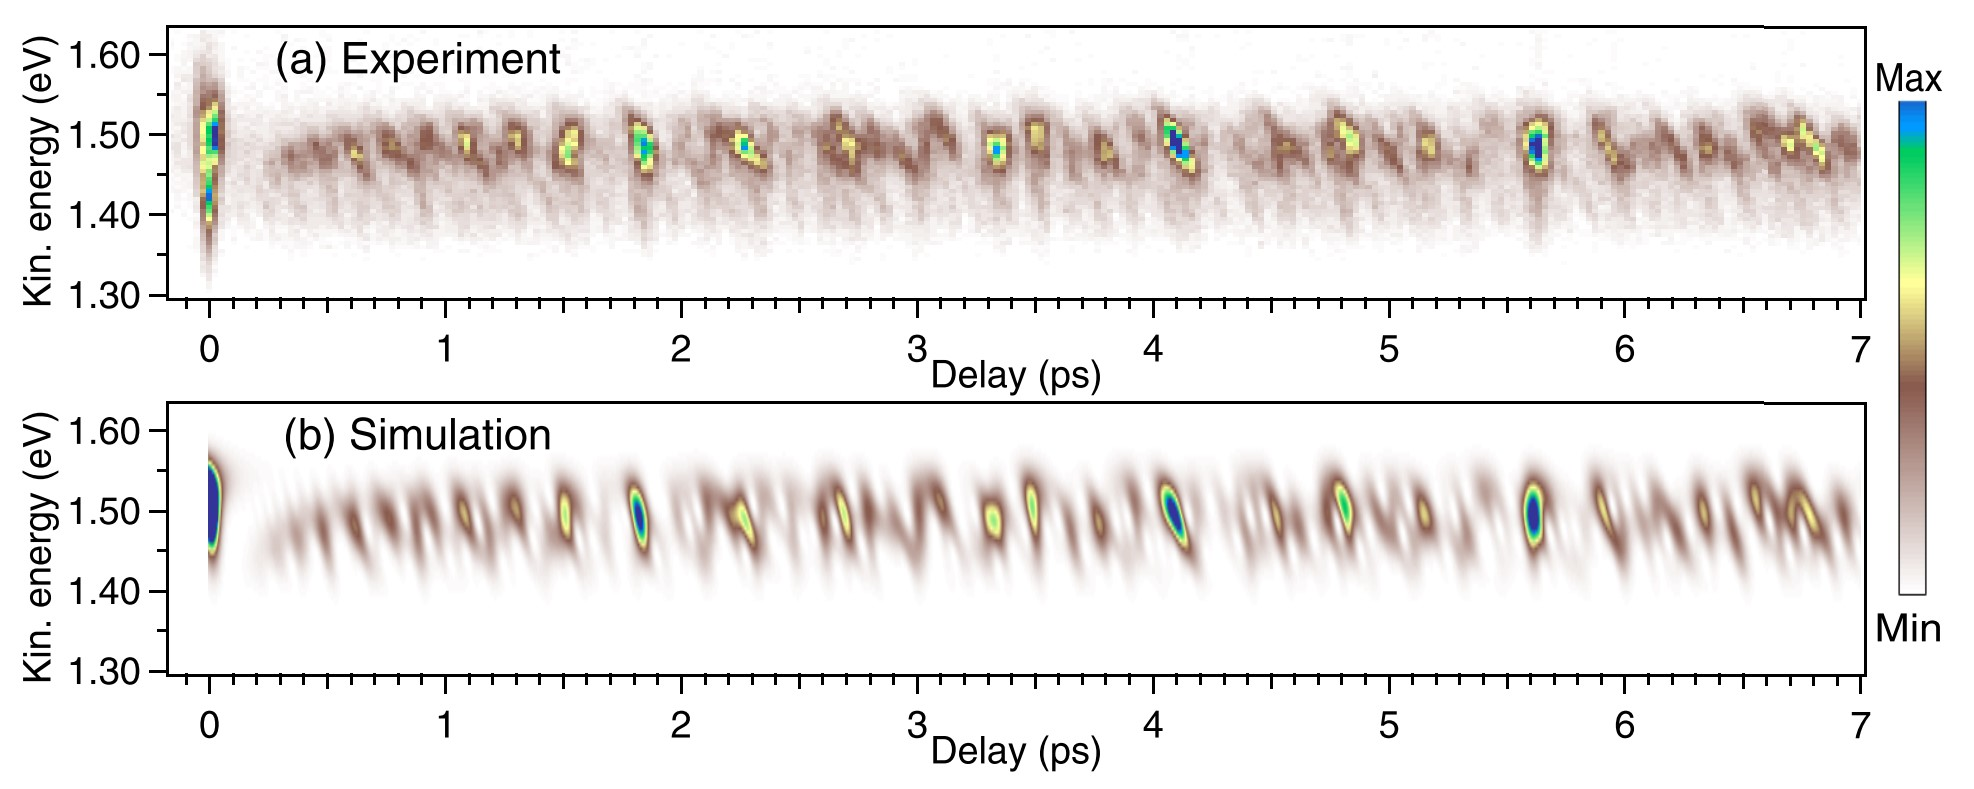
\includegraphics[scale= .34]{Imagenes/Grafica 1 pagina 4.jpg}
    \caption*{\small{FIG. 2. (a) Experimental photoelectron yield map as a function of the delay between XUV and NIR pulses. (b) Simulated photoelectron yield map using 24.587 eV XUV central energy and 0.09433 eV XUV bandwidth.
 }}
    \label{grafica 1 pagina 4}
\end{figure}


\begin{multicols}{2}

\small{}


as “correct points.” The length of the slices varied between
0.7 and 3 ps. The results are presented in Fig. 4(a). For slices
ranging from 1.7 to 3 ps, the correct time is found in 100\%
of the cases. Shortening the length of the slices worsens the
result, e.g., 0.7 ps slice shows correct match only in 41.7\% of
cases.

In Fig. 4(b) we show the time difference between the
QUBS-time and the DS-time for the case of 2 ps slices. It is
clear that there is a linear increase in the time difference with
increasing delay. This is consistent with the conclusion that
the drift is due to a misalignment of the delay stage

To conclude, we have shown that it is possible to obtain
quantitative correspondence between experiment and theory
for a complex wave packet containing multiple Rydberg
states. This can be used for verifying calculated values of the
quantum defect since small deviations of the QD will result in
large deviations of the time-dependent electron yield at large
delays. Note that a photoelectron analyzer is not necessary, i.e., it is enough to measure the total photoelectron yield, as
long as a bias is applied for blocking low-kinetic-energy electrons. Furthermore, we have shown that a 1.7 ps slice of the
photoelectron yield is long enough to uniquely determine how
much time has passed since the wave packet was formed. This
is with the assumption that the measurement never exceeds
10 ns. For the 100 ns time range, a 3 ps window is needed for
a unique determination of the time. We have defined two different timescales, first is the conventional delay stage derived
values of the time (DS-time). The second is the time as given
by quasiunique beat signatures (QUBS-time). In Fig. 3(d),
the experiment and theory are in quantitative agreement. This
proves that the derived QUBS-time is accurate and that any
deviation with the DS-time necessarily indicates an inaccurate
DS-time.

Since high-level Rydberg states can reach lifetimes of well
above microseconds, the QUBS can be used as an artifact-free
watch over a broad time range with an accuracy in the range

\end{multicols}

\begin{figure}[h]
    \centering
    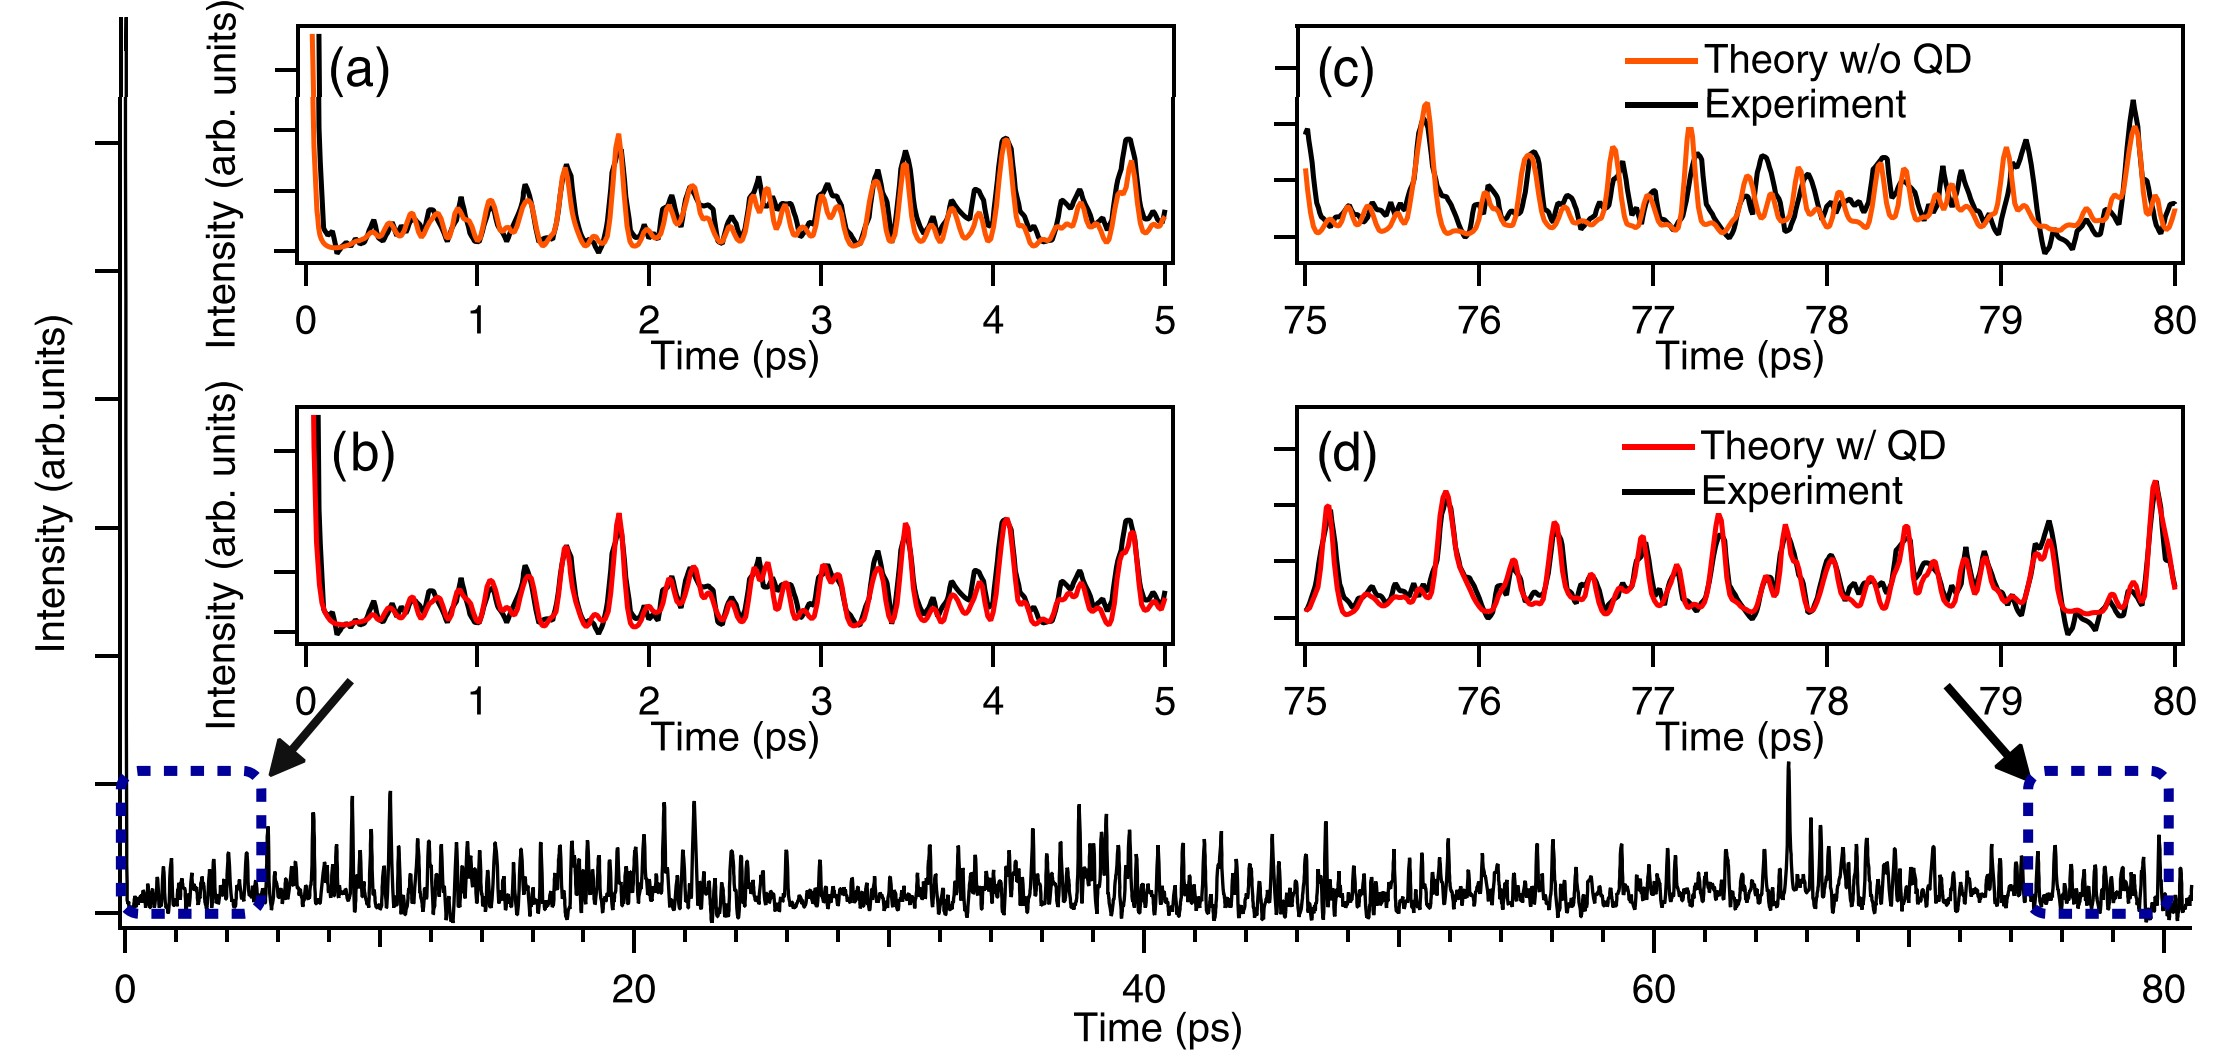
\includegraphics[scale= .37]{Imagenes/GRAFICA 2 pagina 4.jpg}
    \caption*{\small{FIG. 3. Experimental energy integrated photoelectron yield (black line) measured between 0 and 81 ps. Insets (a) and (b) show the section between 0 and 5 ps. Panels (c) and (d) show the section between 75 and 80 ps. Simulated results are shown with orange and red lines. Simulations in (a) and (c) are performed without any QD, while (b) and (d) have included the QD. Simulations were performed using 24.6208 eV XUV center energy with a FWHM of 0.0944 eV.
 }}
    \label{grafica 2 pagina 4}
\end{figure}



%--------------CABECERA--------
\newpage
\fancyhead[C]{ } 
\fancyhead[L]{\scriptsize{QUANTUM WATCH AND ITS INTRINSIC PROOF OF …}} 
\fancyhead[R]{\scriptsize{PHYSICAL REVIEW RESEARCH \textbf{4}, 043041 (2022)}}
\fancyfoot[L]{}
\fancyfoot[C]{ \footnotesize{043041-5}}
\fancyfoot[R]{ }
%--------------------------------
\begin{multicols}{2}
    

    \begin{Figura}
     \centering
    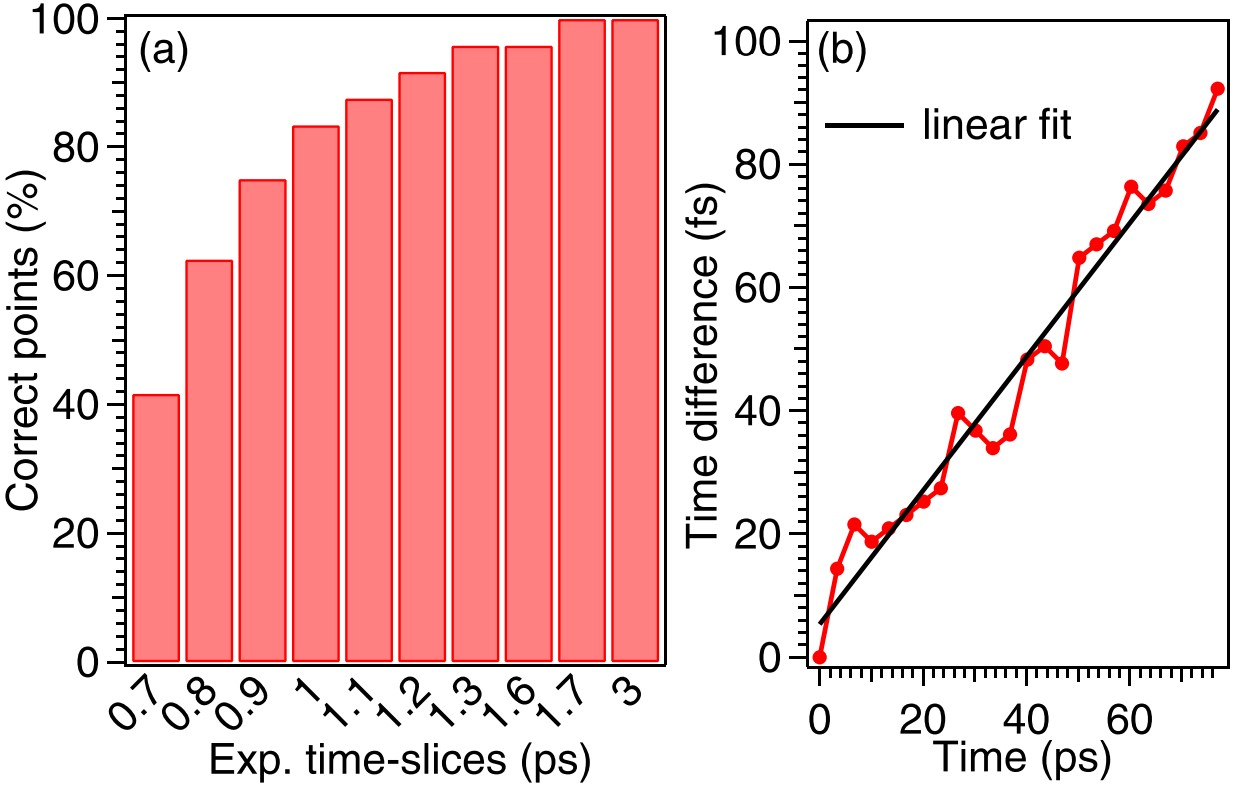
\includegraphics[scale= .37]{Imagenes/grafica 1 pagina 5.jpg}
    \label{grafica 1 pagina 5}   
    \end{Figura}

    \small{}
    
   FIG. 4. (a) The proportion of experimental slices, with different lengths, that were assigned a correct time delay when compared to a 10 ns simulated range. (b) The difference between QUBS-time and DS-time for 24 slices that are 2 ps long, with starting point given by the horizontal axis.\\
\newline
of femtoseconds. The accuracy of the QUBS-time can be considered twofold, first is the quality of the experimental data and to which accuracy it can be fitted to the theoretical data. We find that the experimental data can be determined within 1 fs using least-squares fits. The second is to what accuracy a QUBS fingerprint determines the QUBS-time. By comparing Figs. 3(c) and 3(d), we see that there is a shift of about 100 fs and a significant change in the structure of the QUBS between using QD and not using QD. This provides an estimate of how well we can determine the QUBS-time. Since the QUBS structure can determine the QD amplitude to within 8\%, we should have similar accuracy for the QUBS-time, i.e., 100 fs × 0.08 = 8 fs.

A quantum watch can be tailored to serve a specific experiment since there are several possibilities in terms of samples and required photon energies. To realize the quantum watch
working principle, in addition to a large ensemble of states in a WP, the states must be long lived. Typically, Rydberg states converging at the ionization potential are very long-lived and therefore suitable to use in the quantum watch application over a broad time range. If one needs to use lower-photonenergy pump pulses, then inert gases such as Ne, Ar, Kr, and Xe could be used instead of He. Increasing the photon energy of the pump pulse is not impossible either, although not trivial. Ions could be used instead of neutral species because of their higher excitation energies. Another option might be to use fluorescence decay of core-excited states to create a WP using x rays. The valence-excited state reached after the fluorescence decay remains as a coherently excited WP and can be used in the same way as described in this paper for direct excitation. However, the implementation could be experimentally challenging due to competing decay mechanisms.

\begin{center}
    {\textbf{ACKNOWLEDGMENTS}}
\end{center}

This work was supported by the Estonian Research Council grant (PUTJD909). M.B. also acknowledges the Centre of Excellence Advanced Materials and High-technology Devices for Sustainable Energetics, Sensorics, and Nanoelectronics TK141.
\end{multicols}

\centering{\rule{87mm}{0.1mm}}

\begin{multicols}{2}

\def\refname{}

\begin{thebibliography}{30} %número total de referencias

\small

\vspace{-7mm}

\bibitem{} A. Stolow, Applications of wavepacket methodology, \href{https://royalsocietypublishing.org/doi/10.1098/rsta.1998.0169}{Philos.
Trans. R. Soc. Lond. A \textbf{356}, 345 (1998).}
\vspace{-1.5mm}

\bibitem{} M. Wollenhaupt, V. Engel, and T. Baumert, Femtosecond laser
photoelectron spectroscopy on atoms and small molecules: Prototype studies in quantum control,  \href{https://www.annualreviews.org/doi/10.1146/annurev.physchem.56.092503.141315}{Annu. Rev. Phys. Chem. \textbf{56},
25 (2005).}
\vspace{-1.5mm}

\bibitem{} G. Alber, H. Ritsch, and P. Zoller, Generation and detection of
Rydberg wave packets by short laser pulses, \href{https://journals.aps.org/pra/abstract/10.1103/PhysRevA.34.1058}{Phys. Rev. A \textbf{34},
1058 (1986).}
\vspace{-1.5mm}

\bibitem{} J. A. Yeazell and C. R. Stroud, Jr., Observation of Spatially
Localized Atomic Electron Wave Packets, \href{https://journals.aps.org/prl/abstract/10.1103/PhysRevLett.60.1494}{Phys. Rev. Lett. \textbf{60},
1494 (1988).}
\vspace{-1.5mm}

\bibitem{} M. Lucchini, A. Ludwig, T. Zimmermann, L. Kasmi, J.
Herrmann, A. Scrinzi, A. S. Landsman, L. Gallmann, and U.
Keller, Anisotropic emission in quantum-beat spectroscopy of
helium excited states, \href{https://journals.aps.org/pra/abstract/10.1103/PhysRevA.91.063406}{Phys. Rev. A \textbf{91}, 063406 (2015).}
\vspace{-1.5mm}

\bibitem{} K. Klünder, P. Johnsson, M. Swoboda, A. L’Huillier, G.
Sansone, M. Nisoli, M. J. J. Vrakking, K. J. Schafer, and J.
Mauritsson, Reconstruction of attosecond electron wave packets using quantum state holography, \href{https://journals.aps.org/pra/abstract/10.1103/PhysRevA.88.033404}{Phys. Rev. A \textbf{88}, 033404
(2013).}
\vspace{-1.5mm}

\bibitem{} M. Lucchini, J. Herrmann, A. Ludwig, R. Locher, M. Sabbar,
L. Gallmann, and U. Keller, Role of electron wavepacket interference in the optical response of helium atoms, \href{https://iopscience.iop.org/article/10.1088/1367-2630/15/10/103010}{New J. Phys.
\textbf{15}, 103010 (2013).}
\vspace{-1.5mm}

\bibitem{} N. Shivaram, H. Timmers, X.-M. Tong, and A. Sandhu,
Attosecond-Resolved Evolution of a Laser-Dressed Helium
Atom: Interfering Excitation Paths and Quantum Phases, \href{https://journals.aps.org/prl/abstract/10.1103/PhysRevLett.108.193002}{Phys.
Rev. Lett. \textbf{108}, 193002 (2012).}
\vspace{-1.5mm}

\bibitem{} P. Ranitovic, X. M. Tong, B. Gramkow, S. De, B. DePaola,
K. P. Singh, W. Cao, M. Magrakvelidze, D. Ray, I. Bocharova,
H. Mashiko, A. Sandhu, E. Gagnon, M. M. Murnane, H. C.
Kapteyn, I. Litvinyuk, and C. L. Cocke, IR-assisted ionization
of helium by attosecond extreme ultraviolet radiation, \href{https://iopscience.iop.org/article/10.1088/1367-2630/12/1/013008}{New J.
Phys. \textbf{12}, 013008 (2010).}
\vspace{-1.5mm}

\bibitem{} P. Johnsson, J. Mauritsson, T. Remetter, A. L’Huillier, and K. J.
Schafer, Attosecond Control of Ionization by Wave-Packet Interference, \href{https://journals.aps.org/prl/abstract/10.1103/PhysRevLett.99.233001}{Phys. Rev. Lett. \textbf{99}, 233001 (2007).}
\vspace{-1.5mm}

\bibitem{} Y. Hikosaka, H. Iwayama, and T. Kaneyasu, Zeeman quantum
beats of helium Rydberg states excited by synchrotron radiation, \href{https://scripts.iucr.org/cgi-bin/paper?S1600577520002829}{J. Synchr. Radiat. \textbf{27}, 675 (2020).}
\vspace{-1.5mm}

\bibitem{} Y. Hikosaka, T. Kaneyasu, M. Fujimoto, H. Iwayama, and M.
Katoh, Coherent control in the extreme ultraviolet and attosecond regime by synchrotron radiation, \href{https://www.nature.com/articles/s41467-019-12978-w}{Nat. Commun. \textbf{10}, 4988}
(2019).
\vspace{-1.5mm}

\bibitem{} J. Mauritsson, T. Remetter, M. Swoboda, K. Klünder, A.
L’Huillier, K. J. Schafer, O. Ghafur, F. Kelkensberg, W. Siu,
P. Johnsson, M. J. J. Vrakking, I. Znakovskaya, T. Uphues, S.
Zherebtsov, M. F. Kling, F. Lépine, E. Benedetti, F. Ferrari,
G. Sansone, and M. Nisoli, Attosecond Electron Spectroscopy
 



%--------------CABECERA--------
\newpage
\fancyhf{}
\fancyhead{}
\thispagestyle{UltimaPagina}

%\fancyhead[C]{} 
%\fancyhead[L]{\footnotesize{MARTA BERHOLTS \emph{et al}}} 
%\fancyhead[R]{\footnotesize{PHYSICAL REVIEW RESEARCH 4, 043041 (2022)}}
%\fancyfoot[L]{}
%\fancyfoot[C]{\footnotesize{043041-6}}
%\fancyfoot[R]{}

%--------------------------------
Using a Novel Interferometric Pump-Probe Technique, \href{https://journals.aps.org/prl/abstract/10.1103/PhysRevLett.105.053001}{Phys. Rev. Lett. \textbf{105}, 053001 (2010).}
\vspace{-1.5mm}

\bibitem{} N. Shivaram, X.-M. Tong, H. Timmers, and A. Sandhu,
Attosecond quantum-beat spectroscopy in helium, \href{https://iopscience.iop.org/article/10.1088/0953-4075/49/5/055601}{J. Phys. B:
At., Mol. Opt. Phys. \textbf{49}, 055601 (2016).}
\vspace{-1.5mm}

\bibitem{} R. Pazourek, M. Reduzzi, P. A. Carpeggiani, G. Sansone, M.
Gaarde, and K. Schafer, Ionization delays in few-cycle-pulse
multiphoton quantum-beat spectroscopy in helium, \href{https://journals.aps.org/pra/abstract/10.1103/PhysRevA.93.023420}{Phys. Rev.
A \textbf{93}, 023420 (2016).}
\vspace{-1.5mm}

\bibitem{} K. T. Kim, Dong Hyuk Ko, J. Park, N. N. Choi, C. M. Kim,
K. L. Ishikawa, J. Lee, and C. H. Nam, Amplitude and Phase
Reconstruction of Electron Wave Packets for Probing Ultrafast Photoionization Dynamics, \href{https://journals.aps.org/prl/abstract/10.1103/PhysRevLett.108.093001}{Phys. Rev. Lett. \textbf{108}, 093001
(2012).}
\vspace{-1.5mm}

\bibitem{} C. E. Theodosiou, Lifetimes of singly excited states in He I,
\href{https://journals.aps.org/pra/abstract/10.1103/PhysRevA.30.2910}{Phys. Rev. A \textbf{30}, 2910 (1984).}
\vspace{-1.5mm}

\bibitem{} G. W. F. Drake, High precision theory of atomic helium, \href{https://iopscience.iop.org/article/10.1238/Physica.Topical.083a00083}{Phys.
Scr. \textbf{T83}, 83 (1999).}
\vspace{-1.5mm}

\bibitem{} A. Kramida, Yu. Ralchenko, J. Reader, and NIST ASD Team,
NIST Atomic Spectra Database (ver. 5.9) (National Institute of
Standards and Technology, Gaithersburg, MD 2021).
\vspace{-1.5mm}

\bibitem{} O. Guyétand, M. Gisselbrecht, A. Huetz, P. Agostini, R. Taeb,
V. Vniard, A. Maquet, L. Antonucci, O. Boyko, C. Valentin, and
D. Douillet, Multicolour above-threshold ionization of helium:
Quantum interference effects in angular distributions, \href{https://iopscience.iop.org/article/10.1088/0953-4075/38/22/L01}{J. Phys.
B: At. Mol. Opt. Phys. \textbf{38}, L357 (2005).}
\vspace{-1.5mm}

\bibitem{} M. Žitnik, A. Stani, K. Bu ar, J. G. Lambourne, F. Penent, R. I.
Hall, and P. Lablanquie, Lifetimes of n 1
P states in helium, \href{https://iopscience.iop.org/article/10.1088/0953-4075/36/20/010}{J.
Phys. B: At. Mol. Opt. Phys. \textbf{36}, 4175 (2003).}
\vspace{-1.5mm}

\bibitem{} M. Larsson, B. Mannfors, and W. R. Pendleton, Radiative lifetimes of 1
S and 1
P Rydberg levels of He, \href{https://journals.aps.org/pra/abstract/10.1103/PhysRevA.28.3371}{Phys. Rev. A \textbf{28}, 3371
(1983).}
\vspace{-1.5mm}

\bibitem{} Edited by G. W. F. Drake, Springer Handbook of Atomic,
Molecular, and Optical Physics (Springer, New York, 2006),
p. 237.
\vspace{-1.5mm}

\bibitem{} V. D. Ovsiannikov, I. L. Glukhov, and E. A. Nekipelov, Ionization cross sections and contributions of continuum to optical
characteristics of Rydberg states, \href{https://iopscience.iop.org/article/10.1088/0953-4075/45/9/095003}{J. Phys. B: At. Mol. Opt. Phys.
\textbf{45}, 095003 (2012).}
\vspace{-1.5mm}

\bibitem{} S. Plogmaker, J. A. Terschlüsen, N. Krebs, M. Svanqvist,
J. Forsberg, U. B. Cappel, J.-E. Rubensson, H. Siegbahn,
and J. Söderström, HELIOS—A laboratory based on highorder harmonic generation of extreme ultraviolet photons for
time-resolved spectroscopy, \href{https://aip.scitation.org/doi/10.1063/1.4937463}{Rev. Sci. Instrum. \textbf{86}, 123107
(2015).}
\vspace{-1.5mm}

\bibitem{} R. Stefanuik, R. Knut, S. Jana, J. A. Terschlüsen, A. Sandell,
and J. Söderström, Developments and enhancements to the
HELIOS pump probe system, \href{https://www.sciencedirect.com/science/article/abs/pii/S0368204817300129?via%3Dihub}{J. Electron Spectrosc. Relat.
Phenom. \textbf{224}, 33 (2018).}
\vspace{-1.5mm}

\bibitem{} R. Budriunas, Collinear setup for two-color high-harmonic generation, Bachelor’s thesis, Lund University, 2012.
\vspace{-1.5mm}

\bibitem{} I. J. Kim, C. M. Kim, H. T. Kim, G. H. Lee, Y. S.
Lee, J. Y. Park, D. J. Cho, and C. H. Nam, Highly Efficient High-Harmonic Generation in an Orthogonally Polarized Two-Color Laser Field, \href{https://journals.aps.org/prl/abstract/10.1103/PhysRevLett.94.243901}{Phys. Rev. Lett. \textbf{94}, 243901
(2005).}
\vspace{-1.5mm}

\bibitem{} J. Mauritsson, P. Johnsson, E. Gustafsson, A. L’Huillier, K. J.
Schafer, and M. B. Gaarde, Attosecond Pulse Trains Generated
using Two Color Laser Fields, \href{https://journals.aps.org/prl/abstract/10.1103/PhysRevLett.97.013001}{Phys. Rev. Lett. \textbf{97}, 013001
(2006).}
\vspace{-1.5mm}

\bibitem{} See Supplemental Material at \url{http://link.aps.org/supplemental/
10.1103/PhysRevResearch.4.043041} for quantum defect fitting
results, Rydberg energies, and quantum defect values used in
this work.


\end{thebibliography}

\end{multicols}

\end{document}
